\section{Diagrammes UML de Connect Four}

\begin{figure}[H]
    \centering
    \begin{tikzpicture}
        \begin{umlsystem}{Connect Four}
            \umlusecase[x=-2,y=5]{TODO add action}
            \umlusecase[x=-2,y=3]{TODO add action}
            \umlusecase[y=1]{TODO add action}
            \umlusecase[y=-1]{TODO add action}
            \umlusecase[x=4,y=4]{TODO add action}
        \end{umlsystem}

        \umlactor[y=2,x=-6]{Actor}

        \umlassoc{Actor}{usecase-1}
        \umlassoc{Actor}{usecase-3}
        \umlassoc{Actor}{usecase-2}
        \umlassoc{Actor}{usecase-4}

        \umlinclude{usecase-1}{usecase-5}
        \umlinclude{usecase-2}{usecase-5}
        \umlextend{usecase-3}{usecase-4}
    \end{tikzpicture}
    \caption{Diagramme de cas d’utilisation UML de haut niveau de Connect Four}
\end{figure}

\begin{figure}[H]
    \centering
    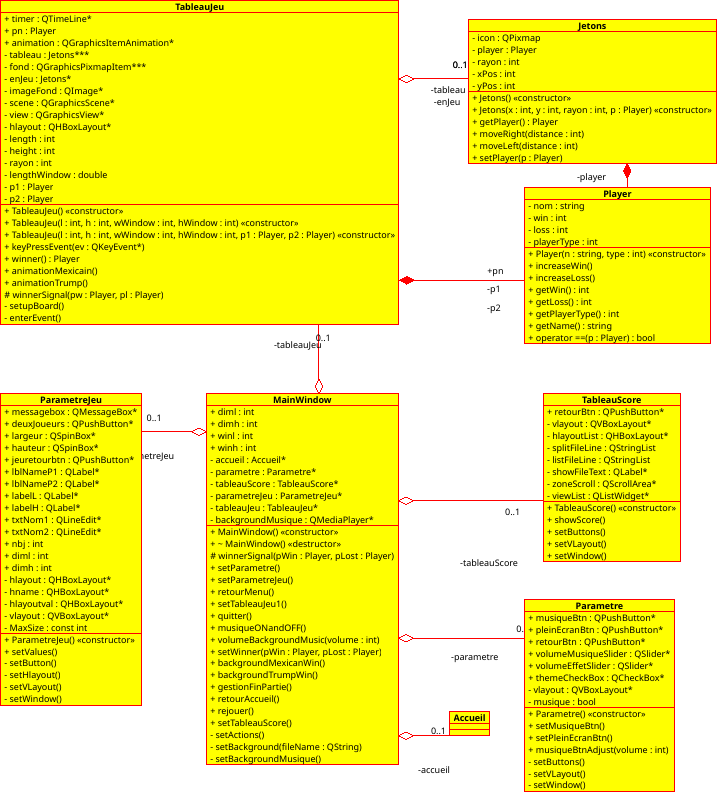
\includegraphics[width=6in]{img/classes}
    \caption{Diagramme de classe de Connect Four}
\end{figure}

\section{Captures d’écrans}

\begin{figure}[H]
    \centering
    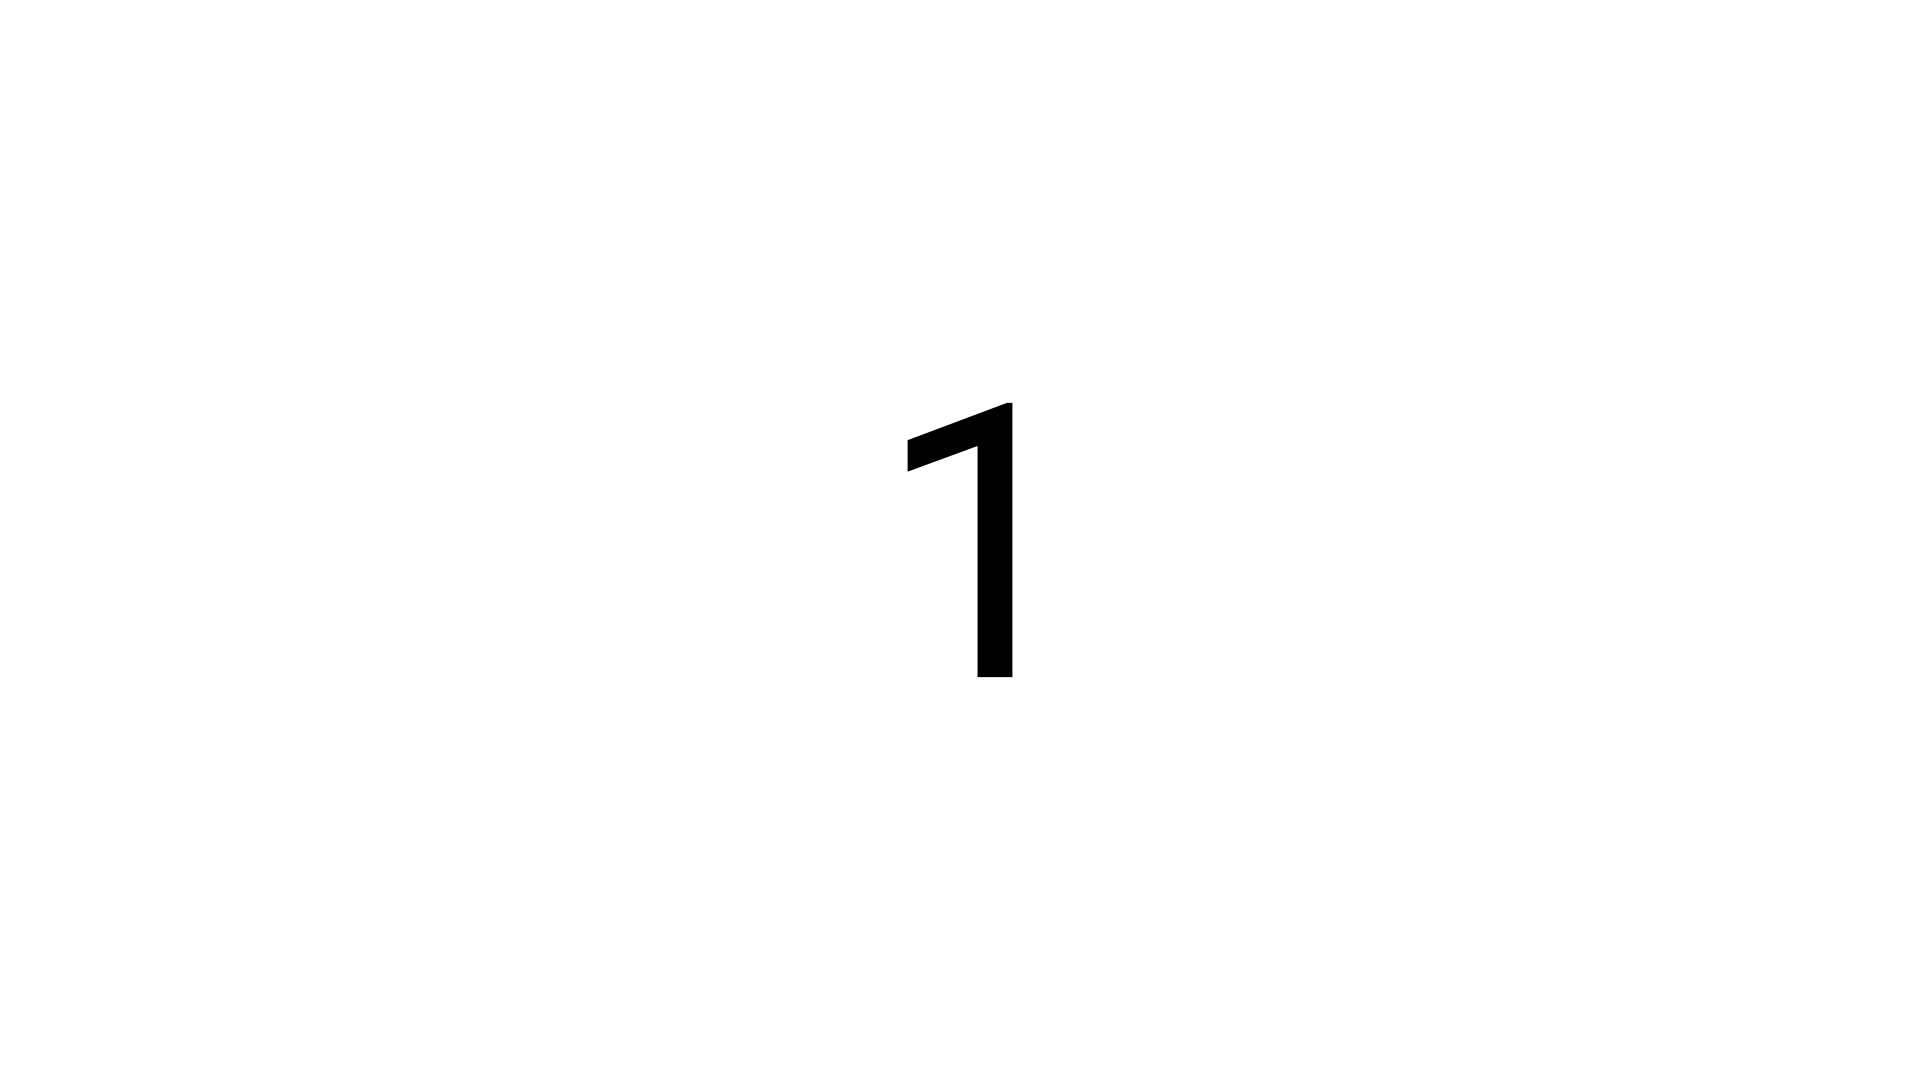
\includegraphics[width=6in]{img/1}
    \caption{Écran 1}
\end{figure}

\begin{figure}[H]
    \centering
    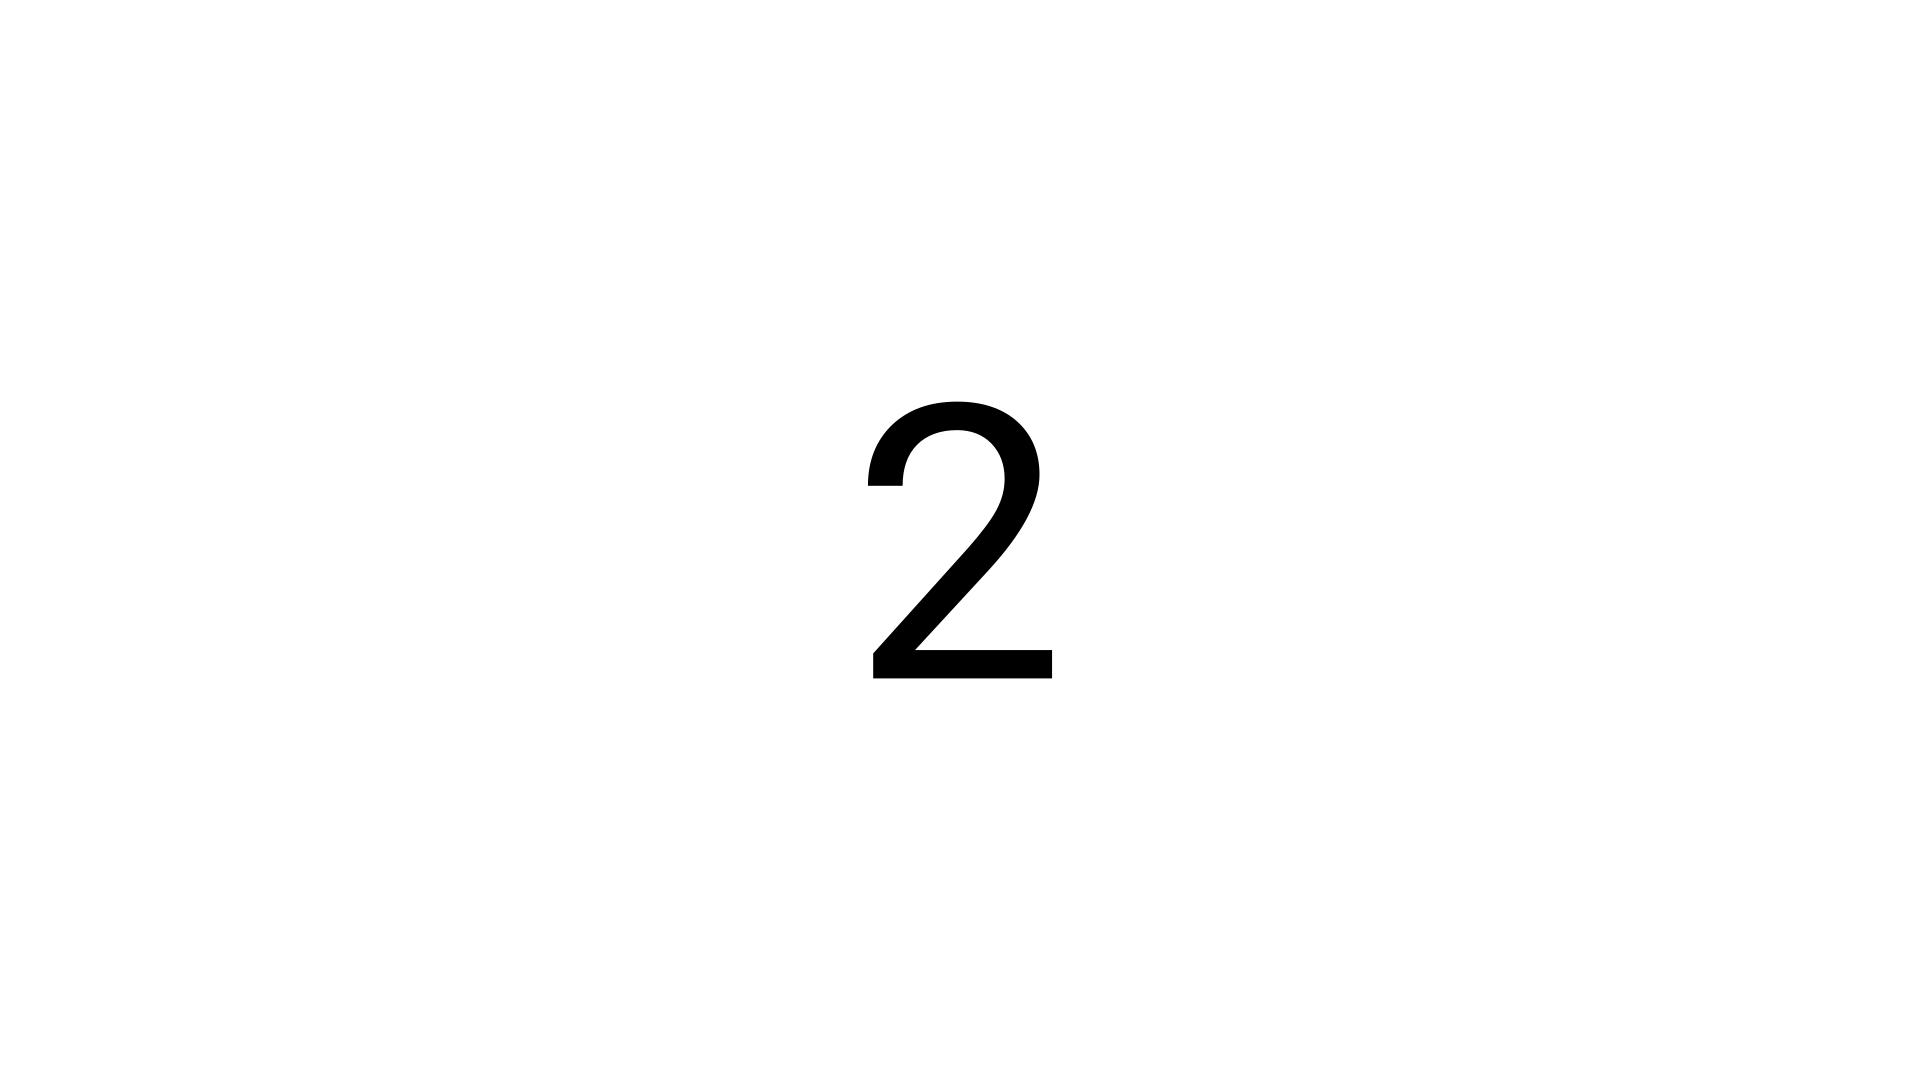
\includegraphics[width=6in]{img/2}
    \caption{Écran 2}
\end{figure}

\begin{figure}[H]
    \centering
    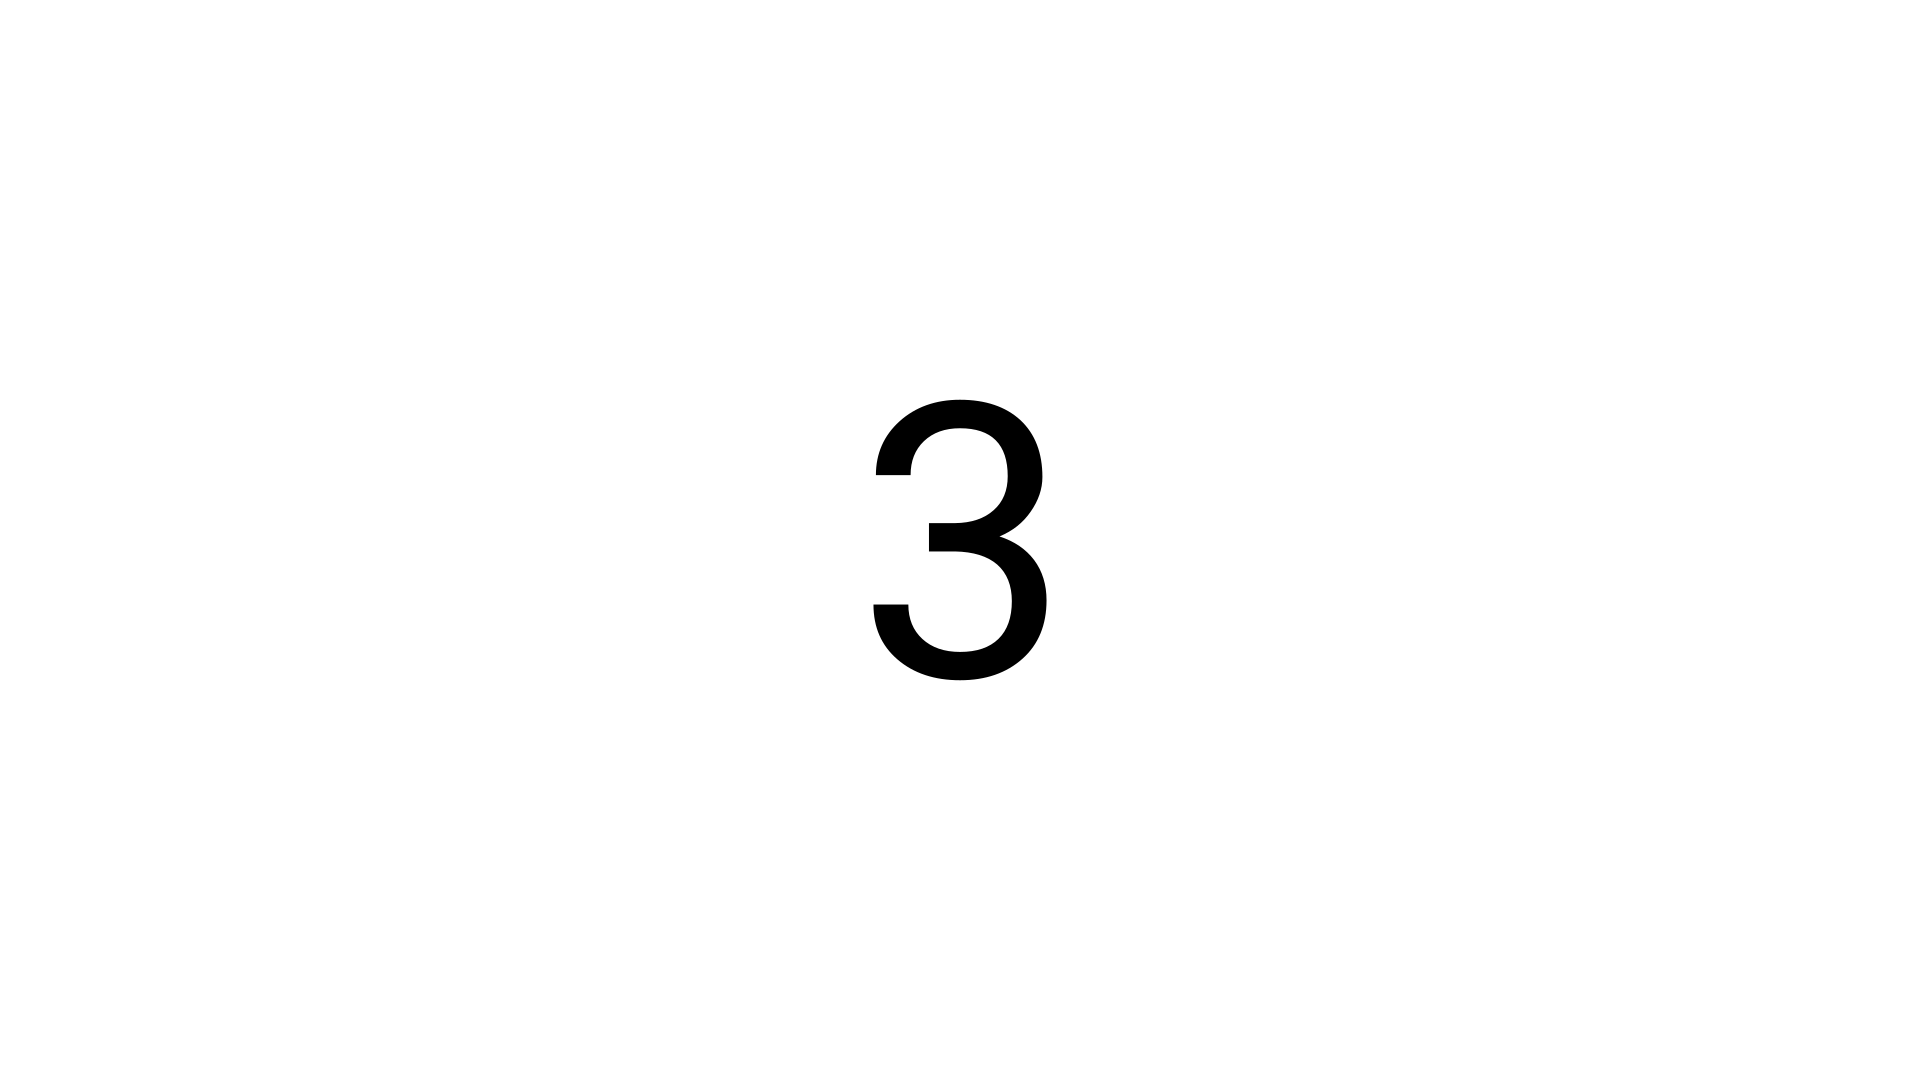
\includegraphics[width=6in]{img/3}
    \caption{Écran 3}
\end{figure}

\begin{figure}[H]
    \centering
    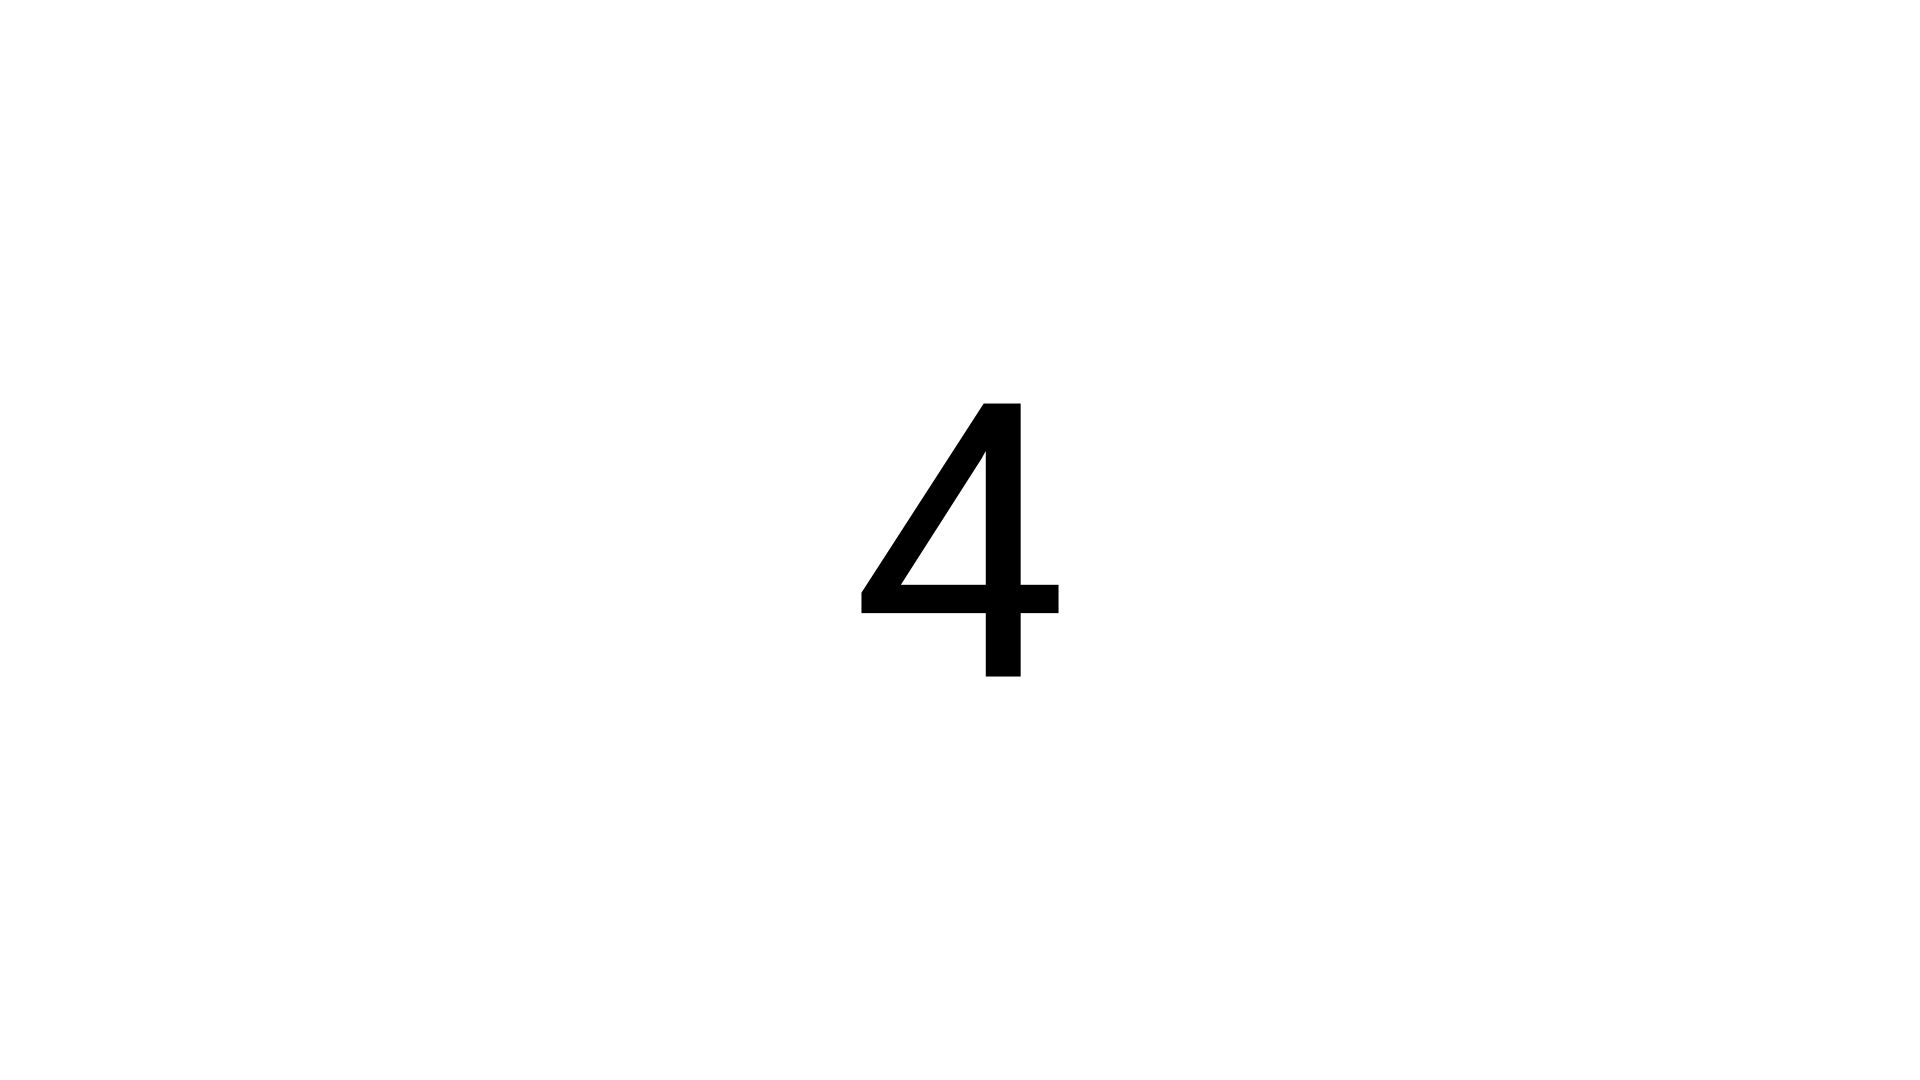
\includegraphics[width=6in]{img/4}
    \caption{Écran 4}
\end{figure}

\section{But, fonctionnement et guide d'usager de Conect Four}

\section{Ergonomie et amélioration}



\section{Plan de tests de Connect Four}

\begin{table}[H]
    \centering
    \caption{Plan de tests de l'interface graphique}
    \begin{tabular}{p{2in}p{2in}p{2in}}
        \hline
        \bfseries Fonction & \bfseries Paramètre & \bfseries Résultat attendu\\
        \hline
        getLargeur & Rectangle() & 1\\
        getHauteur & Rectangle() & 1\\
        getAncrage & Rectangle() & \{0, 0\}\\
        aire & Rectangle() & 1\\
        \hline
        getLargeur & Rectangle(2, 3, \{4, 5\}) & 2\\
        getHauteur & Rectangle(2, 3, \{4, 5\}) & 3\\
        getAncrage & Rectangle(2, 3, \{4, 5\}) & \{4, 5\}\\
        aire & Rectangle(2, 3, \{4, 5\}) & 6\\
        \hline
    \end{tabular}
\end{table}

\begin{table}[H]
    \centering
    \caption{Plan de tests de l'application}
    \begin{tabular}{p{2in}p{2in}p{2in}}
        \hline
        \bfseries Fonction & \bfseries Paramètre & \bfseries Résultat attendu\\
        \hline
        getLargeur & Rectangle() & 1\\
        getHauteur & Rectangle() & 1\\
        getAncrage & Rectangle() & \{0, 0\}\\
        aire & Rectangle() & 1\\
        \hline
        getLargeur & Rectangle(2, 3, \{4, 5\}) & 2\\
        getHauteur & Rectangle(2, 3, \{4, 5\}) & 3\\
        getAncrage & Rectangle(2, 3, \{4, 5\}) & \{4, 5\}\\
        aire & Rectangle(2, 3, \{4, 5\}) & 6\\
        \hline
    \end{tabular}
\end{table}
